\lhead{\emph{\leftmark}}  

\chapter{Detection Mechanisms for UML/Umple Constructs}
\label{chap:detections}

In this chapter, we will present the different mechanisms to detect UML/Umple attributes, associations and state machines from source code written in an object-oriented programming language. We started to build our detection rules based on the following:

\begin{enumerate}

\item Documented implementations of attributes and associations in high-level programming languages mentioned in the literature. In particular, we have considered research that discusses how to generate code from these modeling concepts (forward engineering).

\item Documented techniques in the literature for discovering  modeling constructs in object-oriented source code (reverse engineering).

\item Our own analysis of open source systems written in object-oriented programming languages.

\end{enumerate}

To present the set of transformation rules derived from our analysis, we  employ a semi-formal notation. The rules define the transformation from input to output. These transformations rules can be described using a metamodel-based language or grammar-based language. Both types of descriptions allow us to specify mappings between source and target models in the form of conditions (patterns) and conversions (replacements) executed from input to output when those conditions hold. As the intent of our work is to transform object-oriented  language programs into Umple programs, we  employ a metamodel-based approach to better express the input/output relationships. The metamodel-based language will be enhanced with OCL \cite{WarmerOCL2003} expressions. 
% create table in chapter 5, showing m2t and m2m requirements in terms of Model source code
% M2M: UmpleModel, JavaModel
% M2T: JavaModel, UmpleCode
% T2T: Java code, Umple Code

\section{A Notation for Transformation Rules}
\label{sec:2ModelTransformation}

Transformation rules presented in this chapter contain the following information:

\begin{enumerate}

\item A name for each transformation rule used for reference purposes.

\item The source language reference.

\item Constants used in the generation of the target.

\item Helper methods used in the extraction of information from target or input models.

\item A set of named source language model elements from the source language metamodel that we call B.

\item A set of named target language model elements from the target language metamodel that we call U.

\item The source language conditions: invariants that state the conditions that must hold in the source model for this transformation to be applied.

\item The target language conditions: invariants that state the conditions that must hold in the target model for this transformation to be applied.

\end{enumerate}

% It would be better in this template if the keyword 'conditions' and 'mappings' would be in blue, just like 'in' and 'out'
% MG Fixed

Listing \ref{lst:templateTransform} presents a template definition for the transformations rules.

\begin{lstlisting}[style=mine,caption=Template definition for transformation rules,label=lst:templateTransform]
Transformation Name  (InputModel, OutputModel){
 order n
 params
 	...
 in
   sourceElement: ...
 out
   targetElement: ...
 in-out conditions
 	...
 mappings
    sourceElement.propertyA -> targetElement.propertyA;
    sourceElement.propertyB -> targetElement.propertyB;
}
\end{lstlisting}

The various parts of a transformation rule have their own  specific notation:

\begin{itemize}

\item Line 1. Every transformation possesses a name. The source and target languages are referenced by stating both language names after the transformation name.

\item Line 2. The order of application of the rule is determined by the integer number following the keyword \textit{order}. Rules with lower order numbers are executed first. Order of application of the rules does not matter when two or more rules possess the same order number. 

\item Line 3. Local and global variables to be used in the transformation rule are specified following the keyword \textit{params}.

\item Lines 5 and 7. The source model and target elements are written as variable declarations following the keywords \textit{in} and \textit{out} respectively.

\item Line 9. The conditions that must hold on the source and target model elements are specified following the keywords \textit{in-out conditions}. The mappings are performed only if all conditions specified are true. Conditions are specified using OCL syntax. 

\item Line 11. The mapping rules come after the keyword \textit{mappings}. The symbol -\textgreater \newline is used as an infix operator with two operands. The symbol specifies a transformation of the left hand side operand to the right side operand (rules are unidirectional).
\end{itemize}

We will now introduce the transformation rules for each of the transformation steps presented in Chapter \ref{chap:core}.
The set of rules for each transformation case constitutes a transformation case definition. Rules in the set are to be executed in sequence.

\section{Transformation Rules for the Initial Transformation Step}

Transformations rules for this step are straightforward and aim at transforming the package declaration, namespace declarations, import declaration and the generalization notation into the corresponding Umple notation. 

The mapping rule in Listing \ref{lst:4.1.1} specifies the transformation of a Class into an Umple class using the language defined in the previous section. A type declaration in the base language model represents an object-oriented type (i.e., a class, interface, struct, etc). The only required condition in the rule shown in Listing \ref{lst:4.1.1} (Line 7) is that the \textit{typeDeclaration} must declare a class and not an interface or abstract class. A very similar rule is then required for the transformation of a \textit{typeDeclaration} into an Umple Interface. The relationship between the source model, the target model and the mapping rule (in blue background) are illustrated in Figure \ref{fig:4.1.1}.
Transformation rules defined in a general but formal language can then be adapted to specific languages such as Java or C++. For instance, the name of a typeDeclaration if the input language is Java can be extracted using the \textit{getName().getFullyQualifiedName()} call sequence. Actual implementation of the mapping rules will be presented in Chapter \ref{chap:tool}. For our first example, we show the BNF grammar for a type declaration in Java and an Umple class declaration in Listings \ref{lst:javaGrammar1} and \ref{lst:umpleGrammar2} respectively. It must be pointed out that the transformation rule can be understood either by looking at the metamodel or the grammar of input/output models. 

% The following Listing is totally mixed up with the subsequent figure in the tool, but when I export a pdf it looks OK. Very strange.
% MG. Strange, I see the same problem. PDF will be fine however.

% Also, you are using tabs, which Latex does not process properly in listings. You need to use two spaces instead of tabs. I have made this change in this case, but make the change elsewhere and watch out in other code.
% Fixed MG.

% Readers will be confused as to the detailed sublanguages (e.g. the reference to isInterface(), ::TypeDeclariation, .name and so on. How are you going to define these? I know you say this is 'informal' (actually I changed it to 'semiformal' which is the correct term), but nonetheless it should be understandable. Are you referring to JDT contstructs? If so then there is the problem that you have not introduced JDT yet. Perhaps the solution is to put much of Chapter 5 before this (discussing how you tried ATL, TXL and then briefly xDT), then have this chapter, which can now refer to JDT, and finally discuss the implification in another separate chapter. There would end up being one more chapter than there is now.
% But there may be another way to make this all make sense, such as defining the semi-formal language in a simple way here.
% MG Fixed by using a more abstract way of presenting the language. 

\begin{lstlisting}[style=mine,caption=Grammar for Java types,label=lst:javaGrammar1]
TypeDeclaration:
                ClassDeclaration
                InterfaceDeclaration
 ClassDeclaration:
      [ Javadoc ] { Modifier } class Name
                        [ extends Type]
                        [ implements Type { , Type } ]
                        { { ClassBodyDeclaration | ; } }
 InterfaceDeclaration:
      [ Javadoc ] { Modifier } interface Identifier
                        [ extends Type { , Type } ]
                        { { InterfaceBodyDeclaration | ; } }
\end{lstlisting}

\begin{lstlisting}[style=mine,caption=Grammar for Umple classes,label=lst:umpleGrammar2]
 umpleClass : class Name { [[classContent]]* }
\end{lstlisting}

\begin{lstlisting}[style=mine,caption=Rule BaseTypeToUmpleClass,label=lst:4.1.1]
Transformation BaseTypeToUmpleClass (BaseLanguageMetamodel, UmpleMetamodel){ 
 in
   typeDeclaration : BaseLanguageModel::TypeDeclaration;
 out
   UmpleClass: UmpleMetamodel::UmpleClass;
 in conditions
   typeDeclaration.oclIsTypeOf(ClassDeclaration);   
 mappings
   typeDeclaration.name -> UmpleClass.name;
}
\end{lstlisting}

\begin{figure}[h]
\centering
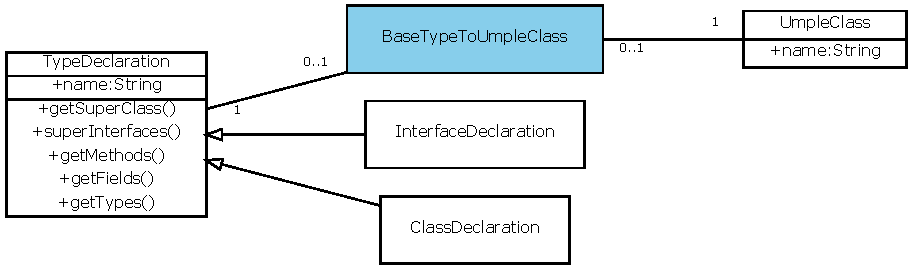
\includegraphics[width=0.99\textwidth]{Figures/ch4InitialMapping.pdf}
\caption{Input-output relationships for rule BaseTypeToUmpleClass}
\label{fig:4.1.1}
\end{figure}

Similarly, rule  \textit{ImportToUmpleDepend} in Listing \ref{lst:4.1.2} specifies the transformation of an import declaration into a depend declaration. Import directives in object-oriented languages are used to incorporate information from a type library. 

\begin{lstlisting}[style=mine,caption=Rule JavaImportToUmpleDepend,label=lst:4.1.2]
Transformation ImportToUmpleDepend (BaseLanguageMetamodel, UmpleMetamodel){ 
 in
   importDeclaration : BaseLanguageModel::ImportDeclaration;
 out
   depend: UmpleMetamodel::Depend;
 in-out conditions
	none
 mappings
   importDeclaration.name -> depend.name;
   fieldDeclaration.importDeclaration -> UmpleClass.depend;
}
\end{lstlisting}

Rule \textit{PackageToUmpleNamespace} in Listing \ref{lst:4.1.3} specifies the transformation of a package declaration into a namespace declaration in Umple. Package declarations in object-oriented languages are used to organize and group classes.

\begin{lstlisting}[style=mine,caption=Rule PackageToUmpleNamespace,label=lst:4.1.3]
Transformation PackageToUmpleNamespace (BaseLanguageMetamodel, UmpleMetamodel){ 
 in
   packageDeclaration : BaseLanguageModel::PackageDeclaration;
 out
   UmpleClass: UmpleMetamodel::UmpleClass;
 in-out conditions
    none
 mappings
   packageDeclaration.name -> UmpleClass.namespace;
}
\end{lstlisting}

Furthermore, the generalization in the base language notation is transformed into the Umple notation \textit{isA} as shown in Listing \ref{lst:4.1.5}.

\begin{lstlisting}[style=mine,caption=Rule GeneralizationToUmpleIsA,label=lst:4.1.5]
Transformation GeneralizationToUmpleIsA (BaseLanguageMetamodel, UmpleMetamodel){ 
 in
   typeDeclaration : BaseLanguageModel::TypeDeclaration;
 out
   UmpleClass: UmpleMetamodel::UmpleClass;
 in conditions
   typeDeclaration.oclIsTypeOf(ClassDeclaration);   
 mappings
   typeDeclaration.superInterfaceTypes -> UmpleClass.parentInterfaces;
   typeDeclaration.superClassType -> UmpleClass.extendsClass;
}
\end{lstlisting}

At this transformation step, we do not attempt to transform any variable into an Umple attribute, association end or state machine. As a result the field declarations and related method declarations are simply appended to the body of the Umple class; some of these will be transformed later. The rule \textit{ClassBodyToUmpleClassExtracode} in Listing \ref{lst:4.1.4} performs the desired operation. We employ the OCL feature \textit{iterate} to traverse the collection of methods and fields belonging to the field declaration. 

\begin{lstlisting}[style=mine,caption=Rule ClassBodyToUmpleClassExtracode,label=lst:4.1.4]
Transformation ClassBodyToUmpleClassExtracode (BaseLanguageMetamodel, UmpleMetamodel){ 
 in
   fieldDeclaration : BaseLanguageModel::FieldDeclaration;
   methodDeclaration : BaseLanguageModel::MethodDeclaration;
   typeDeclaration : BaseLanguageModel::TypeDeclaration;
 out
   UmpleClass: UmpleMetamodel::UmpleClass;
 in conditions
   typeDeclaration.oclIsTypeOf(ClassDeclaration);   
 mappings
   typeDeclaration->iterate( f: FieldDeclaration | 
     fieldDeclaration.toString -> UmpleClass.extraCode);
   methodDeclaration->iterate( f: FieldDeclaration | 
     fieldDeclaration.toString -> UmpleClass.extraCode);
}
\end{lstlisting}

Rules aiming at transforming type declarations into Umple interfaces are very similar to those presented above except that now the `in-out' condition becomes: 
\newline
`\textit{oclIsTypeOf(InterfaceDeclaration)}'.

Finally, enumerations are umplified into Umple `enums'. An \textit{enum} in Umple is a state machine that has events.

\section{Member Variables Analysis}
Member variables can represent not only attributes, but also associations, state machine variables, and internal data such as counters, caching, or sharing of local data. In this section, we analyze the characteristics of member variables and present the mapping rules guiding the transformation of
these member variables into attributes or associations variables. Furthermore, we analyze the different patterns supported by existing reverse engineering tools when it comes to the detection of these UML/Umple constructs. 

\subsection{Transformations Rules to Create Attributes}
%FINAL CHANGE START
The first part of our analysis, as stated at the beginning of this Chapter, consists of analyzing how real projects implement attributes. In previous work done by co-researchers \cite{UmpleAttributes} seven projects picked randomly from open source repositories were studied. The seven projects included: from GoogleCode: fizzbuzz, ExcelLibrary, ndependencyinjection and Java Bug Reporting Tool; from SourceForge: jEdit and Freemaker; and from Freecode (formerly Freshmeat): Java Financial Library.
Refer to Table \ref{table:umplifiedSystems} for details about the systems. 
%LAST added reference to table in chapter 6
%FINAL CHANGE END

From these projects, we identified 1831 member variables in the 469 classes analyzed. From the member variables found, 1211 were instance variables and 620 were class (static) variables. The results of this study showed that:

\begin{itemize}
\item 27\% of the instance variables were of a number type. This includes primitive integers, unsigned and signed numbers.
\item 14\% of the instance variables were of a string type. 
\item 10\% of the instance variables were of Boolean type.
\item 2\% of the instance variables were of Date and Double type.
\item 47\% of the instance variables were of a different data type (reference type).
\end{itemize}

As discussed in Chapter \ref{chap:core} and presented in the study done by co-researchers \cite{UmpleAttributes}, the type of an (candidate) attribute is either a simple data type such as the types in Table \ref{table:attributes2} or a class that contains itself only instance variables of primitive type. The latter case is illustrated through Listings \ref{lst:PersonCandidateAttr}-\ref{lst:AddressCandidateAttr}. In the example, the class \textit{Address} (a reference type) contains only instance variables of primitive type and therefore is more likely an attribute. 

\begin{table}
\caption{Umple primitive data types}
\label{table:attributes2}
\centering
    \begin{tabular}{ll}
		\toprule
		\rowcolor[HTML]{BBDAFF}
        \textbf{Type}      & \textbf{Description}                               \\ 
        \hline
        Integer   & Includes signed and unsigned integers.    \\ 
        String    & All string and string builder types       \\ 
        Boolean   & true/false types                          \\ 
        Double    & All decimal object types                  \\ 
        Date/Time & All date, time and calendar object types. \\
        \hline
    \end{tabular}
\end{table}

\noindent\begin{minipage}{.45\textwidth}
\begin{lstlisting}[style=java,caption=Person.java,label=lst:PersonCandidateAttr]{Name}
public class Person {
 private Address address;
 // ... Other parts omitted
}
\end{lstlisting}
\end{minipage}\hfill
\begin{minipage}{.45\textwidth}
\begin{lstlisting}[style=java,caption=Address.java,label=lst:AddressCandidateAttr]{Name}
public class Person {
 // ... Other parts omitted
 // Getters, setters and constructors omitted
 private String postalCode;
 private int streetNumber;
 private String streetName;
 private int apptNumber;
}
\end{lstlisting}
\end{minipage}

Candidate attributes, those instance variables possessing the characteristics mentioned above, are further analyzed. The instance variables were analyzed for their presence in constructors and in and get/set methods. This is a key fact that helped us determine whether the member variable can indeed become an Umple attribute. Table \ref{table:attributesAnalysis} presents the results for this part of the study.
Those instance variables with high and medium probability are definitely attributes. The instance variables with a low or very low probability of being attributes are not transformed for now. 

\begin{table}[h]
\caption{Analyzing instance variables for presence in the constructor and getter/setters}
\label{table:attributesAnalysis}
\centering
\begin{tabular}{@{}cccc@{}}
\toprule
\rowcolor[HTML]{BBDAFF}
\multicolumn{1}{c}{\cellcolor[HTML]{BBDAFF}\textbf{Constructor}} & \multicolumn{1}{c}{\cellcolor[HTML]{BBDAFF}\textbf{Setter}} & \multicolumn{1}{c}{\cellcolor[HTML]{BBDAFF}\textbf{Getter}} & \multicolumn{1}{c}{\cellcolor[HTML]{BBDAFF}\begin{tabular}[c]{@{}c@{}}\textbf{Attribute}\\ \textbf{(Probability})\end{tabular}} \\ \midrule
Yes                                                     & Yes                                                & Yes                                                & High                                                                                                          \\
Yes                                                     & Yes                                                & No                                                 & Low                                                                                                           \\
Yes                                                     & No                                                 & Yes                                                & High                                                                                                          \\
Yes                                                     & No                                                 & No                                                 & Low                                                                                                           \\
No                                                      & Yes                                                & Yes                                                & High                                                                                                          \\
No                                                      & Yes                                                & No                                                 & Low                                                                                                           \\
No                                                      & No                                                 & Yes                                                & Medium                                                                                                        \\
No                                                      & No                                                 & No                                                 & Very Low                                                                                                      \\ \bottomrule
\end{tabular}
\end{table}

As presented in Chapter \ref{chap:background}, attributes can be categorized into 4 main categories: \textit{lazy}, fully editable, derived or immutable. By analyzing the presence of the variable in the constructor, getter and setter we can determine to which of the categories the extracted attributes belongs to. Table \ref{table:constructorFrequency} presents the different categories of attributes and whether or not they are required as arguments in the constructor, getter and setters. Lazy attributes for instance are those with postponed initialization (third line in Table \ref{table:constructorFrequency}). Therefore, when the member variable 
\begin{enumerate*}
  \item has a \textit{Get} method,
  \item has a \textit{Set} method and
  \item is not one of arguments of the constructor 
\end{enumerate*}, it is matched (converted) into a lazy Umple attribute. 

\begin{table}
\caption{Type of attribute based on their presence in constructor and access method patterns}
\label{table:constructorFrequency}
\centering
\begin{tabular}{llll}
\toprule
\rowcolor[HTML]{BBDAFF}
\textbf{Type}   & \textbf{Contructor}    & \textbf{Setter}       &  \textbf{Getter} \\ 
\hline
 Fully editable & Yes & Yes & Yes \\
  Immutable & Yes & No & Yes \\
   Lazy & No & Yes & Yes \\
    Derived & No & No & Yes \\
\hline
\end{tabular}
\end{table}

Results of the first part of the analysis on the seven open-source projects can be found at:
\url{https://github.com/mgarzon/experiments/mgarzon/thesis/CH4Detection}.

The second part of our analysis of attributes consisted of reviewing how other reverse engineering tools 
recover attributes from source code. Reverse engineering tools in Table \ref{table:toolsReverse} were employed to recover attributes from (Java) source code. Since all the tools mentioned above generate UML models from source code (and not Umple models) we are not concerned here about the `lazyness' or `immutability' characteristics of the attributes. In fact, we are only concerned about the following:

\begin{table}[h]
\caption{Reverse-engineering tools evaluated}
\label{table:toolsReverse}
\centering
\begin{tabular}{lll}
\toprule
\rowcolor[HTML]{BBDAFF}
\textbf{Tool}   & \textbf{Version}  & \textbf{Type}\\ 
\hline
 ArgoUML \cite{ArgoUML} & 0.32.2 & Open-source \\
 Intellij IDEA \cite{IdeaTool} & 14.1 & Commercial \\
 Visual Paradigm \cite{VisualParadigm} & 12.0 & Commercial  \\
 Rational Rose Modeler  \cite{ROSE} & 7.1 & Commercial\\
 Fujaba \cite{Fujaba} & (Reclipse) 1.0 & Research\\
 Ptidej \cite{ptidejTool} & 5.8 & Research\\
\hline
\end{tabular}
\end{table}

\begin{enumerate}
\item Is the tool able to correctly recover the type of the attribute?

\item Is the tool able to distinguish cases in which the member variable is of a reference type but that type contains itself only variables of primitive type? It is a correct recovery if the member variable is extracted as an attribute and not as an association (one-to-one)?

\item Is the tool able to distinguish a `local variable' from a real attribute by analyzing the presence of an accessor/mutator in the source code?  It is a correct recovery if only member variables possessing a getter are recovered as attributes. 

\item Is the tool able to deal with all the many different ways of coding an accessor/mutator? `N/A' in this context means that the tool does not analyze constructors, mutators or accessors when recovering attributes. 

\item Is the tool able to distinguish between one (0..1 or 1) and many (*) based on the attribute type? It is a correct recovery if list structures and object types with a plural noun were identified as \textit{many}, all other structures should be identified as \textit{one}. An example of an attribute with  \textit{many} multiplicity is `List\textless String \textgreater ids'.

\item Is the tool able to recover class level attributes (i.e. static)?
\end{enumerate}

Table \ref{table:analyzeAttributesSecondPart} presents the results.

\begin{table}[h]
\caption{Analysis of reverse-engineering tools for the recovery of attributes}
\label{table:analyzeAttributesSecondPart}
\centering
\begin{tabular}{lllllll}
\toprule
\rowcolor[HTML]{BBDAFF}
\textbf{Tool}   & \textbf{1}    & \textbf{2}   &  \textbf{3}   &  \textbf{4} &  \textbf{5}  &  \textbf{6} \\ 
\hline
ArgoUML & Yes & No & No & N/A & No & Yes\\ 
IDEA & Yes & No & No & No & No  & Yes\\ 
Visual Paradigm & Yes & No & Yes & No & No & Yes \\ 
Rational Rose & Yes & Yes & No & No & Yes & Yes\\ 
Fujaba & Yes & Yes & No & Yes & Yes & Yes\\ 
Ptidej & Yes & Yes & No & N/A & Yes & Yes\\ 
\hline
\end{tabular}
\end{table}

By analyzing existing projects and assessing how reverse engineering tools recover attributes, we were able to align our detection mechanisms (mapping rules) with the observed trends, and ensure our tool fills in the gaps that other tools leave.

The mapping rules obtained from our analysis are presented next.

\begin{lstlisting}[style=mine,caption=Case 1 - Variable has a getter ,label=lst:attrCase1]
Transformation FieldToUmpleBasicAttribute (BaseLanguageMetamodel, UmpleMetamodel){ 
 in
   fieldDecl : BaseLanguageModel::FieldDeclaration;
 out
   attr: UmpleMetamodel::Attribute;
 in-out conditions
 	fieldDecl.type.oclIsTypeOf(PrimitiveType) 
 	   OR fieldDecl.type.oclIsTypeOf(ComplexType) ;
 	hasAGetter(fieldDecl);
 mappings
    fieldDecl.name -> attr.name;
    fieldDecl.type -> attr.type;
}
\end{lstlisting}

\begin{lstlisting}[style=mine,caption=Is a fully editable attribute,label=lst:attrCase2]
Transformation FieldToUmpleFullAttribute (BaseLanguageMetamodel, UmpleMetamodel){ 
 in
   fieldDecl : BaseLanguageModel::FieldDeclaration;
 out
   attr: UmpleMetamodel::Attribute;
 in-out conditions
 	fieldDecl.type.oclIsTypeOf(PrimitiveType)
 	    | fieldDecl.type.oclIsTypeOf(ComplexType);
 	hasAGetter(fieldDecl);
 	hasASetter(fieldDecl);
 	hasAConstructor(fieldDecl);
 mappings
    fieldDecl.name -> attr.name;
    fieldDecl.type -> attr.type;
}
\end{lstlisting}

\begin{lstlisting}[style=mine,caption=Is an immutable attribute,label=lst:attrCase3]
Transformation FieldToUmpleImmutableAttribute (BaseLanguageMetamodel, UmpleMetamodel){ 
 in
   fieldDecl : BaseLanguageModel::FieldDeclaration;
 out
   attr: UmpleMetamodel::Attribute;
 in-out conditions
 	fieldDecl.type.oclIsTypeOf(PrimitiveType)
 	 | fieldDecl.type.oclIsTypeOf(ComplexType);
 	hasAGetter(fieldDecl);
 	hasASetter(fieldDecl)==false;
 	hasAConstructor(fieldDecl);
 mappings
    fieldDecl.name -> attr.name;
    fieldDecl.type -> attr.type;
}
\end{lstlisting}

\begin{lstlisting}[style=mine,caption=Is a lazy attribute,label=lst:attrCase4]
Transformation FieldToUmpleLazyAttribute (BaseLanguageMetamodel, UmpleMetamodel){ 
 in
   fieldDecl : BaseLanguageModel::FieldDeclaration;
 out
   attr: UmpleMetamodel::Attribute;
 in-out conditions
 	fieldDecl.type.oclIsTypeOf(PrimitiveType)
 	   | fieldDecl.type.oclIsTypeOf(ComplexType);
 	hasAGetter(fieldDecl);
 	hasASetter(fieldDecl);
 	hasAConstructor(fieldDecl)==false;
 mappings
    fieldDecl.name -> attr.name;
    fieldDecl.type -> attr.type;
}
\end{lstlisting}

These high-level rules are implemented in the Drools language and presented in Chapter \ref{chap:technology}.
In the next section, we will consider associations. 

\subsection{Refactoring to Create Associations}

As we presented in our empirical study that analyzed the generation and extraction of attributes, we discuss in this section associations in practice. We employ the same systems (7) presented in the previous section. From the analysis of finding attributes, we know now which of the instance variables assessed are attributes. The remaining 235 member variables are considered as candidate association ends. In our previous work \cite{UmpleAssociations}, the distribution of the mutator, accessor and availability in constructors were tracked. The study showed that:

\begin{itemize}
\item 29\% of the 235 member variables had both a Get and Set method
\item 38\% of the 235 member variables had at least a Set method (without a Get method)
\item 51\% of the 235 member variables had at least a Get method (without a Set method)
\item 23\% of the 235 member variables did not have a Set method
\item 17\% of the 235 member variables had only a Get method
\item 17.9\% of the 235 member variables provided Add and Remove methods
\end{itemize}

In addition, 42 of the 235 member variables were defined using one of the classes that operate on collections such as Map, Set, Hashtable or List classes and hence likely represented associations with an upper bound greater than one. According to previous work done by co-researchers \cite{UmpleAssociations}, five association patterns categorized by multiplicity were extracted after analyzing 1800 modeled associations in UML diagrams of real systems (MARTE, Flow Composition, ECA, Java, Patterns and rCOS UML profiles) and UML models from our own repository of examples \cite{umpleexamples}. The five association patterns, ordered according to their frequency of usage, are presented below:

\begin{enumerate}
\item one to many (1--*)
\item optional-one to many (0..1--*)
\item many-to-many (*--*)
\item optional-one to one (0..1--1)
\item optional-one to optional-one to optional-one (0..1--0..1)
\end{enumerate}

As it concerns the evaluation of the reverse engineering tools in Table \ref{table:toolsReverse} when it comes to extract associations from source code, we have used our repository of Umple models \cite{umpleexamples} as test cases.  Each of the examples has been reverse-engineered by the different tools allowing us to determine whether or not the tools support the different multiplicity patterns. Note that Java code has been generated from the various Umple examples. Results are presented in Table \ref{table:analyzeAssocsSecondPart}. The outcomes of our evaluation are:

\begin{itemize}
 \item \textbf{Full}: The association multiplicity is correctly extracted from the different Java systems.
 \item \textbf{Partial}: The association multiplicity is correctly extracted in most cases.
 \item \textbf{None}: The association multiplicity is not supported at all.
\end{itemize} 

\begin{table} [h]
\caption{Analysis of reverse-engineering tools for the recovery of associations}
\label{table:analyzeAssocsSecondPart}
\centering
\begin{tabular}{llllll}
\toprule
\rowcolor[HTML]{BBDAFF}
\textbf{Tool}   & \textbf{1--*}    & \textbf{0..1--*}   &  \textbf{*--*}   &  \textbf{0..1--1} & \textbf{0..1--0..1} \\ 
\hline
ArgoUML & Partial & None & Partial & Partial & None \\ 
IDEA & Full & Partial & Full & Partial & Partial \\ 
Visual Paradigm  & Full & Full & Full & Partial & Partial \\ 
Rational Rose & Full & Full & Full & Full & Partial \\ 
Fujaba  & Partial & Partial & Partial & Partial & Partial \\ 
Ptidej  & Full & Partial & Full & Partial & Full \\ 
\hline
\end{tabular}
\end{table}

Based on the findings from our study, we now discuss how the umplification technique infers associations from source code (Transformation 2b). More specifically, we discuss how our technique infers all the fields that represent associations including the role name, association ends, multiplicities and directionality.

As seen in Chapter \ref{chap:core}, a variable represents an association if all of the following conditions apply:
\begin{itemize}
\item Its declared type is a Reference type (generally a class in the current system).
\item The variable field is simple, or the variable field is a container (also known as a collection).
\item The class in which the variable is declared, stores, accesses and/or manipulates instances of the variable type.
\end{itemize}

In the Umplificator, the tool we will describe in Chapter \ref{chap:technology}, these conditions are expressed as rules. The transformation of variables into associations involves a considerable number of transformations and code manipulations. In order to guarantee the correct extraction of an association and to avoid false-negative cases, we consider not only the getter and setter of the fields but also the iteration call sequences (iterators). Table \ref{table:accessors} and Table \ref{table:mutators} present the list of methods considered (parsed and analyzed) in order to infer associations. These methods can be categorized as mutator and accessor methods. In the tables, W is the name of the class at the other end of the association. We have considered those collections of elements defined using Map, Set, List and Hashtable classes (from the Java collections framework or the Standard Template Library in C++).

\begin{table}
\caption{Accessor methods parsed and analyzed}
\label{table:accessors}
\centering
\begin{tabular}{ll}
\toprule
\rowcolor[HTML]{BBDAFF}
\textbf{Method Signature}   & \textbf{Description}                               \\ 
\hline
W getW()  		& Returns the W    \\ 
W getW(index)   & Picks a specific linked W   \\ 
List\textless W\textgreater getWs()   & Returns immutable list of links  \\ 
\hline
\end{tabular}
\end{table}

\begin{table}
\caption{Mutator methods parsed and analyzed}
\label{table:mutators}
\centering
    \begin{tabular}{ll}
		\toprule
		\rowcolor[HTML]{BBDAFF}
        \textbf{Method Signature}   & \textbf{Description}    \\ 
        \hline
        boolean setW(W)   & Adds a link to existing W   		\\ 
        W addW(args)    & Constructs a new W and adds link      \\ 
        boolean addW(W)  & Adds a link to existing W            \\ 
        boolean setWs(W…)    & Adds a set of links              \\ 
        boolean removeW(W) &   Removes link to W if possible    \\
        \hline
    \end{tabular}
\end{table}

\paragraph*{Inferring role names}

Roles names can be easily inferred from the field name. This does not impose a challenge since the field name is always visible during static analysis of source code.

\paragraph*{Inferring directionality}

To infer the directionality of the association, we consider both classes linked by the association. Bi-directionality means that each class can access the linked object(s) of the other class. In the case one of the classes involved in the association cannot access the linked objects of the other class (member variable is not present) the association is declared as unidirectional.

\paragraph*{Inferring multiplicities}

The process of inferring multiplicities from source code starts by analyzing the fields. If the field is an array, or a collection, the multiplicity is many `0..*'. If the field is not an array or collection, the multiplicity is `0..1'. To infer the other multiplicity patterns, analyses of constructors, mutators and accessor methods need to be performed.
%FINAL CHANGE START
Recovery of multiplicities in the umplification approach ignores all constraints involving lower-bound (n) and upper-bound (m) since that would require either \textit{dynamically} counting the number of instances created \cite{Kollmann2001} or parsing arbitrary algorithmic code.
%FINAL CHANGE END
%TLFINAL adjusted to add a few more words since constraints might be detectable statically in certain conditions
More specifically, Table \ref{table:patternsElements} presents the code elements that need to be inspected in order to infer the different patterns.

\begin{table}
\caption{Code elements parsed and analyzed for the different patterns}
\label{table:patternsElements}
\centering
    \begin{tabular}{ll}
		\toprule
		\rowcolor[HTML]{BBDAFF}
        \textbf{Pattern}   & \textbf{Elements Parsed/Analyzed}   \\ 
        \hline
		1  &     Constructor. \\ 
		0..1 &  Set or Get methods. \\ 
		0..* &  Set/Get or Add/Remove methods.\\ 
		1..*  & Constructor.\\ 
        \hline
    \end{tabular}
\end{table}

Other special cases were taking into account when dealing with associations with an upper-bound greater than one. For instance, in Java code created prior to the introduction generics (i.e. Java 1.4), it was not necessary to typecast  objects as much as it was afterwards. For this reason, we need to inspect the add or remove methods to determine the type of object contained (added or removed) by the collection. Most of the other tools we have briefly discussed in this chapter lack mechanisms to infer the type held by a collection.
For instance, a model reverse-engineered from Java 1.4 might, in some tools, result in a one-to-one association between \textit{Mentor} and \textit{List} when in reality the association should be a one-to-many association between \textit{Mentor} and \textit{Student}.

The mapping rules obtained from our analysis are summarized in Table \ref{table:assocsRules} and implemented in Chapter \ref{chap:technology}. Helper functions (in light blue) are also presented in the Table. 

\begin{table}[h]
\caption{Summary of mapping rules for the detection of associations in code, that will be converted into Umple associations}
\label{table:assocsRules}
\centering
	\begin{tabular}{l|p{8cm}}
		\toprule
		\rowcolor[HTML]{BBDAFF}
        \textbf{Rule Name} & \textbf{Description}  \\ \midrule
        isAssociation & Base case rule. Returns an association variable with basic information.  \\ \hline
        isOneToUnknownAssociation & Extracts the multiplicity from one of the ends. Updates the association variable.  \\ \hline
        isManyToUnknownAssociation &  Extracts the multiplicity from one of the ends. The conditions that must hold for this rule to be applied specify that the upper bound is greater than one. Updates the association variable.  \\ \hline
        isOptionalManyToUnknownAssociation & Extracts the multiplicity from one of the ends. Uses other functions to retrieve the lower bound. \\ \hline
        isOptionalOneToUnknownAssociation & Extracts the multiplicity from one of the ends. Uses other functions to retrieve the lower bound. \\ \hline
        MatchOtherAssociationEnd & Attempts to relate associations ends. Returns an association. \\ \hline
        isNavigable & Updates the navigability of the the association by inspecting both association ends.  \\ \hline
        isCustomMethodDeclaration & Returns a code injection required to adapt the existing method declaration.\\ \hline
        isCustomConstructor  & Returns a code injection required to adapt the existing constructor.  
\\ \hline
\rowcolor{aliceblue} 
        isAssociationEndExternal & Returns true if one of the classes involved in the association is not available. See description of external classes in Chapter \ref{chap:background}.
\\   \hline
\rowcolor{aliceblue} 
        isVariableInConstructor & Returns true if the member variable is in the class constructor.
\\    \hline
\rowcolor{aliceblue}  
        hasVariableGetter & Returns true if the member variable possesses a getter. 
\\   \hline     
\rowcolor{aliceblue}
        hasVariableSetter & Returns true if the member variable possesses a setter. 
\\    \hline     
\rowcolor{aliceblue}  
		getTypeOfCollection& Returns the type contained in a collection. 
\\    \hline       
\rowcolor{aliceblue} 
		resetExtraCode & Searches for code that is not required and needs to be removed (fields, methods, constructors) from classes. 
\\  \hline
\rowcolor{aliceblue} 
 		refactorMethod & Uses code injections gathered from other rules/functions to refactor methods.\\ 
\bottomrule
\end{tabular}
\end{table}


\section{Summary}

This chapter  studied how attributes and associations are used in practice; and investigated how these modeling abstractions can be extracted by analyzing source code. We reviewed
the capabilities possessed by various reverse-engineering tools for detecting these model elements. 

We identified various  combinations of multiplicity for association ends and analyzed their impact on code generation and reverse engineering. 

Finally, we presented the  mapping rules for the detection of constructs in source code, focusing on Java.

In the next chapter, we show more concretely how these rules have been implemented in this research.


